




% Antar begreper qknn har blitt intodusert

Now that a parallel k-d tree build algorithm has been build, lets start looking into a parallelization of the qkNN operation. Some question immediately arise. What is the best way to parallelize such a problem? Will a GPU version give a beneficial speedup? This leads to a new resource question that acts as an expatiation of RQ~\ref{rq:serial-kd-tree}.


\begin{myrq}
\label{rq:parallel_query}
    It is possible to parallelize the qkNN query algorithm, in such a way that it gives a significant speed improvement compared to the serial algorithm.
\end{myrq}


To investigate RQ~\ref{rq:parallel_query}, a real world test and implementation is always beneficial, but first some resource and discussion is needed. Especially in what kind of parallelization strategy and algorithm that should be used. Maybe the GPU is not the right way to parallelize this kind of operations.


\subsection{Parallelization strategy} % (fold)
\label{sub:parallelization_strategy}


The problem at hand is the qkNN search, which is where an assumed big number of query's is to be performed on a k-d tree. At first glance this looks good in terms of parallelization. The main task is naturally divided into individual subtasks, namely the queries. This is a perfect parallelization example, where any number of threads independently can move up and down a constant tree structure.

When CUDA and implementation related questions is introduced, some interesting aspects needs to be addressed. The first is how the work should be divided in terms of CUDA resourced. Should one query be done in a block, should each thread to one query or maybe we should use one thread per $k$ in a query. To address this question, one need to be able to determent if a query itself can be parallelized.

First we see that a query does not have many node visits compared to the size and presumably the number of queries. This ratio is based on the binary logarithm, as for example a tree with one million elements and a $k$ equals one, the number of visited nodes is proportional to $20$. This indicated that many threads is not as beneficial. The relative hard problem of parallelize a query is also a good indicator. Parallelization is, as we have discussed earlier, dependent on individual subtask. The query task is heavily dependent, as the next node is determinant on the previous node. The only place independence comes into existents is where left and right subtree is to be searched, but if this is parallelized the benefit of the pruning is partially destroyed. This leads to one conclusion, if threads is not to be wastefully used, one thread per query is required. In terms of independent tasks, the one thread approach is also logical, since the number of queries should outperform the number of cores on the GPU\@.

The overall parallelization strategy is therefore to use one thread per query and equally distribute the queries amongst the GPU's SM\@.


\subsection{Problem with the recursive implementation} % (fold)
\label{sub:problem_with_the_recursive_implementation}

As discussed in previous sections, GPU's and recursion don't get along well. Previously some drawbacks were mentioned, including the disability for thread communication. Since our parallelization strategy new states that all threads do individually work and don't need to communicate, is there steal a reason for a iterative conversion.

One aspect to consider is connected to how the GPU hardware is constructed. The GPU have a lot of lightweight threads, and has therefor not as mush local space or caching as in a CPU\@. This means that the call stack, where the instructions are manged, is relatively small. A recursive algorithm adds instructions on this call stack at each recursive call. This is the reason why the executions flow of a recursive algorithm is hidden, the call stack is not reachable from the programmers point of view. The big question here is wherever the call stack on a CUDA GPU is big enough for our application.

This question was investigated by a trail and error method, since its hard to do the explicit calculations. The call stack is located locally, so results from a block should be enough. To test the limitations a test that spawned $64$ theoretical threads on an increasing tree size should be sufficient. As the tree size passed \numprint{1e5}, we stared to get unknown errors from CUDA\@. This we concluded was the leak of call stack space and concluded that CUDA had a to small call stack for our purpose.


Divergence is also an accept to consider, and in this case execution divergence. This is, as mention before, then the execution of threads in a warp differs. In a recursive algorithm the decision of whether a recursive call should be made or not, is entirely up to a single thread. Once two threads have made different desiccation, there is no guaranty that they will stay in sync.

The execution divergence can be solved by en iterative solution, where one is guaranteed that every thread always stay in sync. An iterative approach will also solve the call stack problem, where the recursion stack is explicitly stored. The transformation is therefor a necessity.


% subsection problem_with_the_recursive_implementation (end)

\subsection{From recursive to iterative implementation} % (fold)
\label{sub:from_recursive_to_iterative_implementation}


To rewrite Algorithm~\ref{alg:recursive_knn_kd_tree_search} into a iterative algorithm by  explicitly managing the recursion stack, some properties about how the search traverse the k-d tree is needed. From Algorithm~\ref{alg:recursive_knn_kd_tree_search} one can see that this is an inorder traversal, since the current node work is node between the recursive calls. This traversal in also the best strategy in a binary tree search, because the pruning of subtrees is maximized. How to make a standard binary search tree in an iterative fashion is described in Cormen\cite[Chapter 12]{Cormen:2001}, but since this is a k-d tree search the implementation is slightly different, as shown in Algorithm~\ref{alg:iterative_knn_kd_tree_search},

\begin{algorithm}
\caption{Iterative kNN k-d tree search}
\label{alg:iterative_knn_kd_tree_search}
\begin{algorithmic}
    \Procedure{Iterative-kNN-KD-Tree}{$K, r, q$}
        \State \text{Let $S$ be a stack for collecting tree nodes}

        \State $i \gets 2$

        \While{$!S.empty$ \textbf{or} $r$ != NIL}
            \If{$r$ = NIL}
                \State $r \gets \Call{Pop}{S}$
                \State $i \gets r.dimension$

                \If{$r.dx^2 < K.max$} \Comment{Can there be closer points in the other subtree?}
                    \State $r \gets r.other$
                \Else
                    \State $r \gets \text{NIL}$
                \EndIf
            \Else
                \State $d \gets \Call{Distance}{r, q}$

                \If{$d < K.max$} \Comment{Is $r$ closer to $q$ than the current k best points?}
                    \State $r.distance \gets d$
                    \State $\Call{Insert}{K, r}$
                \EndIf

                \State $i \gets (i + 1) \bmod k$ \Comment{k = 3 for a three dimensional k-d tree}

                \State $r.dimention \gets i$
                \State $r.dx \gets r.x(i) - q.x(i)$

                \If{$r.dx > 0$}  \Comment{Select $t$ and $o$ so we traverse towards closest point first}
                    \State $t \gets r.left$, $r.other \gets r.right$
                \Else
                    \State $t \gets r.right$, $r.other \gets r.left$
                \EndIf

                \State $\Call{Push}{S, r}$
                \State $r \gets t$
            \EndIf

        \EndWhile
    \EndProcedure
\end{algorithmic}
\end{algorithm}

The algorithm works in the same way as the recursive algorithm, but adds a stack, $S$, called the s-stack, and a while loop in order to handle the tree traversal iteratively. While there is a element assigned to the root variable, $r$, the algorithm will traverse down the target branch, updating the dimension, $i$, calculating the distance, $dx$, determining the target, $t$, and other, $o$, child node. Then it will collect $r$, $o$, $i$ and $dx$ into one element, and push it on the s-stack. Finally the root variable is assigned to the target child, or NIL if we have reached the end of a branch.

While there still is elements in the s-stack, but $r$ is assigned to NIL, we are traversing back up a branch. While this is happening, the algorithm pops elements from the s-stack, determines if they should be added to the k-heap, before it determines if it need to investigate the other branch of this node. If that is the case, the other node is assigned to $r$, and the algorithm will traverse down this subtree using the previously stated rules.


% subsection from_recursive_to_iterative_implementation (end)

%TODO: Forandre header?
\subsection{Our implementation} % (fold)
\label{sub:our_implementation}

To convert our iterative search algorithm to CUDA should now be a trivial matter. The code itself does not need to be parallelized, as only one thread is used per query. Some key aspects is wort highlighting.


As we converted the algorithm from a recursive to a iterative stack based solution, a lot of the problematic divergence was taken avoided. But as shown in Algorithm~\ref{alg:iterative_knn_kd_tree_search}, there is steal some divergence. This is inevitable since the target subtree and other subtree needs to be treated differently. Although, there are possibilities to minimize the thread branching. If threads in a warp is traversing completely different parts of the tree, they will access different nodes. This is called data divergence. They will also be a minimal change for the threads to synchronize there target and other traversing. The solution is to let each warp search for points that are close in 3-d space, which will force the threads to traverse fore or less together. In our application, query for all points in the k-d tree, this is an easy task. When the k-d tree was build the points are, due to the data structure and the nature of a k-d tree, grouped together relatively to their position in space. The divergence will therefore be minimized if the points are fed to the search as they are placed in the k-d tree.


The transformation from a hidden recursive stack to a explicit stack makes a interesting question about where to store the new stack, especially
since it definitely would have overfilled the local call stack space. This is data that are modifiable and thread independent, which means that the memory options are shared memory, texture memory and global memory. First of all, global memory is a working candidate. It has enough space, it is modifiable and accessible to all threads. The huge drawback is the access time, it takes around $400$ clock cycles(Trenger vi cite), and it would be beneficial to use some other kind of memory. Shared memory would be a perfect candidate, because the memory is fast and the need to communicate between blocks is nonexistent. The only needed drawback to address the the amount of data available in shared memory, which is default around $49 kb$ for each block on current NVIDIA GPU's.

The two stacks in question is the k-stack and the transformed recursive stack, called stack from now on. Both stacks are memory wise dependent on number of threads, since each thread needs unique stacks. The stack is dependent on how many elements the inorder tree traversal needs to store. If one looks on how the algorithm handles the stack, one can see that elements are pushed on the way down, and poped when one traverse upwards.  This means that the stack never will be longer then the tree hight, which is the binary logarithm if the size. One stack elemtnt uses $16$ bytes of space, which means that the stack memory is s subset of $\Theta(16\log_2(n)T)$. Here $T$ represent the number of threads and $n$ is the k-d tree size. The k-stack depends on the number of closest neighbors, $k$, and one element uses $8$ bytes. This implies that it uses memory usage will look like, $\Theta(8kT)$.


\begin{figure}[ht!]
\centering
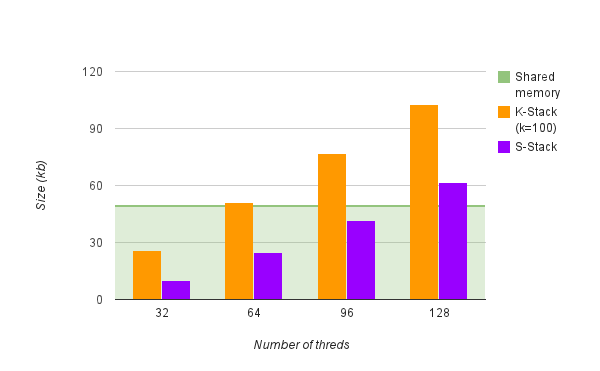
\includegraphics[width=100mm]{../gfx/shared_memory_and_stack.png}

\caption{The stacks memory usage compared to the amount of shared memory.}
\label{fig:stacks_and_shared_memory}
\end{figure}


In Figure~\ref{fig:stacks_and_shared_memory} the memory usage of each stack is compared to the available shared memory. Some basic assumptions and approximations have been done in regard to the data. Treads are only compared in multiples of $32$, since this is the warp size and is therefore the most optimal thread numbers. The value of $k$ is dependent on the problem in hand, and as our application only needs a value of $100$, that value is used. When it comes to the logarithm in the stack calculations, we have chosen $30$.  This is because it value is relatively constant and with a value of this type we support a \numprint{1e9} big k-d tree.


Figure~\ref{fig:stacks_and_shared_memory} shows that the k-stack is not a suitable candidate. The reason is that with $k$ equals $100$ we can only launch one warp per thread. Even though only one warp is pick, the highly dependent and variably $k$ make the stack size to unpredictable. The stack however is looks really promising, with $64$ threads the memory usage is well below the limit.







Memory --> stack  --> openmp
p
cpu vs opemp


% subsection our_implementation (end)





% subsection parallelization_strategy (end)






% \begin{figure}[ht!]
% \centering
% 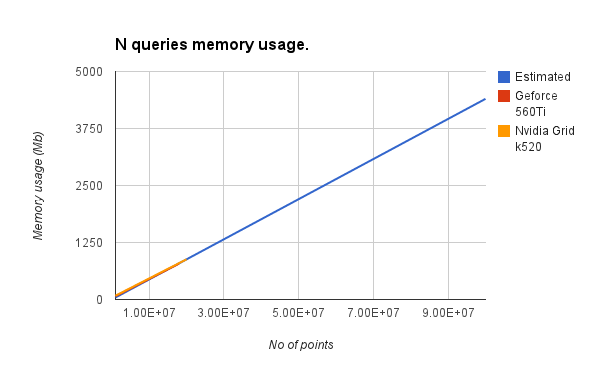
\includegraphics[width=120mm]{../gfx/memory-usage-kd-search.png}

% \caption{Memory usage of kd-search.}
% \label{fig:memory-usage-kd-search}
% \end{figure}

% Also in this case our estimation fit the real consumption with a high degree of accur
% Further work:
% \begin{itemize}
%     \item Look at memory optimization.
%     \item Improve utiliti methods like: accumulateindex, minReduce.
%     \item Forloop Unrolling.
% \end{itemize}



